\clearpage
\subsection{Task 1: ระบบคัดกรองผู้เล่นโกงเบื้องต้น (Anti-Cheat Pre-Filter)}
\label{subsec:task1}

\subsubsection{\texorpdfstring{บริบททางธุรกิจและกลไกของ Metric Binary $F_2$}{บริบททางธุรกิจและกลไกของ Metric Binary F2}}

ภารกิจที่ 1 มุ่งแก้ปัญหาคอขวดเชิงปฏิบัติการของระบบตรวจจับการโกง (Anti-Cheat) ในเครือเกมของ Karena Thailand ปัจจุบันบริษัทได้รับรายงานผู้เล่นต้องสงสัยมากกว่า $10,000$ รายการต่อวัน แต่ทีมตรวจสอบบัญชีด้วยตนเอง (Manual Review) รองรับได้เพียง $500$ เคสต่อวัน ส่งผลให้เกิดรายงานค้างสะสม (Backlog) มากกว่า $45,000$ รายการ ขณะเดียวกันระบบกฎอัตโนมัติแบบเดิมมีอัตราการแจ้งเตือนผิดพลาด (False-Positive Rate) สูงถึง $70\%$ ทำให้ผู้เล่นบริสุทธิ์ถูกระงับบัญชีและสูญเสียความเชื่อมั่น ส่วนผู้โกงระดับสูงที่ใช้โปรแกรมช่วยเล็งแบบแนบเนียน (Subtle Aimbot) หรือมองทะลุกำแพง (Wallhack) กลับเล็ดลอดระบบตรวจสอบ ผลกระทบดังกล่าวนำไปสู่การลดลงของอัตราการรักษาผู้เล่น (Player Retention) ในโหมดแข่งขันถึง $15\%$ และสร้างความเสียหายต่อรายได้ราว $15$ ล้านบาทต่อวัน

ชุดข้อมูลของ Task 1 ประกอบด้วยข้อมูลฝึกสอน (\feat{train.csv}) จำนวน $104,000$ แถว แบ่งเป็นแถวที่มีป้ายกำกับ (\feat{is\_cheater} $\in \{0, 1\}$) จำนวน $90,816$ แถว (ผู้โกง $31,725$ ราย หรือ $34.93\%$ และผู้เล่นปกติ $59,091$ ราย หรือ $65.07\%$) และแถวที่ไม่มีป้ายกำกับจำนวน $13,184$ แถว ($12.68\%$) ส่วนชุดทดสอบ (\feat{test.csv}) มีจำนวน $25,889$ แถว โดยมีฟีเจอร์ดิบเชิงตัวเลขทั้งหมด $31$ คอลัมน์ (ไม่นับ \feat{player\_id} และตัวแปรเป้าหมาย)

เป้าหมายเชิงธุรกิจต้องการระบบคัดกรองเบื้องต้น (Pre-Filter) ที่ไม่ปล่อยให้ผู้โกงตัวจริงหลุดรอด ขณะที่ผลบวกลวงในขั้นคัดกรองยังถูกกลั่นกรองซ้ำโดยผู้ตรวจสอบหรือระบบย่อยถัดไปได้ ดังนั้นเกณฑ์ประเมินจึงใช้ค่า $F_\beta$ ที่ $\beta = 2$ ซึ่งให้น้ำหนักกับ Recall เป็น $4$ เท่า ($\beta^2 = 4$) ของ Precision:
\begin{equation}
F_\beta = \frac{(1+\beta^2)\cdot \text{Precision}\cdot \text{Recall}}{\beta^2\cdot \text{Precision}+\text{Recall}}, \qquad
F_2 = \frac{5\,TP}{5\,TP + 4\,FN + FP}
\label{eq:t1_f2}
\end{equation}
จากสมการ~\eqref{eq:t1_f2} ค่า False Negative ($FN$) ถูกปรับน้ำหนักความเสียหายสูงกว่า False Positive ($FP$) ถึง $4$ เท่า ประเด็นสำคัญเชิงวิศวกรรมที่ส่งผลต่อคะแนนอย่างมีนัยสำคัญคือความแตกต่างระหว่าง \textbf{Macro-$F_2$} (เฉลี่ย $F_2$ ของคลาส $1$ และคลาส $0$ แบบไม่ถ่วงน้ำหนัก) กับ \textbf{Binary-$F_2$} (คำนวณ $F_2$ เฉพาะคลาสผู้โกง \feat{is\_cheater} $= 1$):
\begin{itemize}
  \item ภายใต้สมมติฐาน \textbf{Macro-$F_2$}: การให้น้ำหนักคลาสปกติเทียบเท่าคลาสผู้โกงบังคับให้จุดตัดเหมาะสมอยู่ใกล้สัดส่วนทำนายบวกประมาณ $41\%$ ($40.5\%$--$41.25\%$ บน \feat{final\_v2} และ $40.7\%$ บน Clean ECDF Blend ซึ่งให้ OOF Macro-$F_2 \approx 0.7831$--$0.7833$)
  \item ภายใต้เกณฑ์จริง \textbf{Binary-$F_2$}: เมื่อไม่มีบทลงโทษจากคลาส $0$ โดยตรง จุดตัดที่เหมาะสมเลื่อนลงไปครอบคลุมแถวทำนายบวกประมาณ $62.4\%$ บน OOF (Clean ECDF Blend ที่จุดตัด $\text{thr} = 0.3769$ ให้ OOF Binary-$F_2 = 0.84007$, $\text{Recall} = 0.9722$, $\text{Precision} = 0.5442$; เทียบกับ \feat{final\_v2} ที่อัตราบวก $62.96\%$ ซึ่งให้ $\text{Recall} \approx 0.974$, $\text{Precision} \approx 0.541$) และให้ผลลัพธ์บนชุดทดสอบที่อัตราทำนายบวก $59.33\%$ ($15,359$ แถว)
\end{itemize}

\subsubsection{ข้อค้นพบจาก EDA และโครงสร้างการสร้างข้อมูล}

การวิเคราะห์เชิงลึกผ่านชุดสคริปต์ตรวจสอบโครงสร้าง (\feat{t1/research/} และ \feat{work/insight/}) เผยกลไกของตัวสร้างข้อมูล (Data Generator) ที่กำหนดทิศทางสถาปัตยกรรมโมเดลทั้งหมด ดังสรุปในกรอบ \textbf{Claim $\rightarrow$ Evidence $\rightarrow$ Implication} ต่อไปนี้

\begin{enumerate}
  \item \textbf{การแยกขาดของ 15 Signal Features และ 16 Noise Features ที่มีสหสัมพันธ์หลอก (Correlated Noise)}
  \begin{itemize}
    \item \emph{Claim}: ฟีเจอร์ดิบ $16$ จาก $31$ คอลัมน์ไม่มีข้อมูลแยกแยะคลาสเลย แม้บางคอลัมน์จะมีความสัมพันธ์เชิงเส้นกับฟีเจอร์สัญญาณก็ตาม
    \item \emph{Evidence}: การวัดค่า $|\text{ROC-AUC} - 0.5|$ รายตัวแปรบนข้อมูลมีป้ายกำกับ $90,816$ แถว (รูปที่~\ref{fig:t1_signal_zones}a) พบว่าฟีเจอร์สัญญาณทั้ง $15$ ตัวมีค่า $|\text{AUC} - 0.5| \ge 0.0106$ นำโดย \feat{reports\_received} ($0.1965$), \feat{crosshair\_placement} ($0.1315$), \feat{kill\_death\_ratio} ($0.0824$), \feat{headshot\_percentage} ($0.0786$) และ \feat{game\_sense\_score} ($0.0723$) ลงมาจนถึง \feat{level\_progression\_speed} ($0.0106$) ขณะที่ฟีเจอร์รบกวนทั้ง $16$ ตัวมีค่า $|\text{AUC} - 0.5| \le 0.0033$ (สูงสุดคือ \feat{input\_consistency\_score} $= 0.0033$, ค่า $p$-value ของการทดสอบ KS $> 0.07$ ทุกตัว) เกิดเป็นช่องว่างการแยกขาดที่ชัดเจนถึง $3.2\times$ นอกจากนี้ฟีเจอร์รบกวนหลายตัวสัมพันธ์กับสัญญาณในอัตราเท่ากันทั้งสองคลาส เช่น \feat{input\_consistency\_score} กับ \feat{reaction\_time\_ms} ($\rho \approx 0.26$), \feat{damage\_per\_round} กับ \feat{win\_rate} และ \feat{first\_blood\_rate} กับ \feat{reaction\_time\_ms} การนำฟีเจอร์ $16$ ตัวนี้ใส่กลับเข้าไปใน baseline ทำให้ OOF ROC-AUC (เฉลี่ย 3 seed) ลดลง $0.00042$ (จาก $0.89244$ เหลือ $0.89202$)
    \item \emph{Implication}: ต้องตัดฟีเจอร์รบกวนทั้ง $16$ ตัวทิ้งตั้งแต่ขั้นตอนเตรียมข้อมูล เพื่อลดการแบ่งกิ่งแบบสุ่ม (Split Dilution) ของต้นไม้ตัดสินใจ
  \end{itemize}

  \item \textbf{โครงสร้างกลุ่มย่อยแบบ Uniform Boxes และปรากฏการณ์ ``Smurf-Like'' ในผู้เล่นใหม่ที่บริสุทธิ์}
  \begin{itemize}
    \item \emph{Claim}: ตัวสร้างข้อมูลสุ่มผู้เล่นจาก $5$ กลุ่มย่อยแบบกล่องสม่ำเสมอ (Uniform Boxes) ร่วมกับค่าทักษะแบบเกาส์เซียน ซึ่งก่อให้เกิดช่วงอายุบัญชีที่เป็นคลาสเดียวแบบบริสุทธิ์ (Class-Exclusive Zones) และสวนทางกับสัญชาตญาณเรื่องความแม่นยำของผู้โกง
    \item \emph{Evidence}: การวิเคราะห์การกระจายตัวใน \feat{work/insight/INSIGHTS.md} แสดงขอบเขตกลุ่มย่อยดังนี้:
      \emph{ผู้เล่นปกติกลุ่มใหม่} (Legit New, อายุ $1$--$110$ วัน) มีเพื่อน $U\{0..49\}$, ถูกรายงาน $U\{10..29\}$, เลเวล $U(28, 100)$, \feat{crosshair\_placement} $U(0.82, 0.96)$;
      \emph{ผู้เล่นปกติทั่วไป} (Legit Regular, $120$--$1000$ วัน) มีเพื่อน $U\{45..249\}$, ถูกรายงาน $U\{5..19\}$;
      \emph{ผู้เล่นปกติระดับเก๋า} (Legit Veteran, $200$--$1500$ วัน) มีเพื่อน $U\{100..349\}$, ถูกรายงาน $U\{5..24\}$, \feat{game\_sense\_score} $+0.04$;
      ส่วน \emph{ผู้โกงอายุน้อย} ($15$--$180$ วัน) มีเพื่อน $U\{10..89\}$, ถูกรายงาน $\frac{2}{3}U\{4..15\} + \frac{1}{3}U\{4..19\}$, เลเวล $U(25, 96)$, \feat{crosshair\_placement} $U(0.80, 0.94)$;
      และ \emph{ผู้โกงอายุมาก} ($200$--$1000$ วัน) มีเพื่อน $U\{60..269\}$ โดยใช้ช่วงรายงาน/เลเวล/crosshair เดียวกัน
      ขอบเขตเหล่านี้สร้างหน้าต่างอายุบัญชีที่บริสุทธิ์ $100\%$ (รูปที่~\ref{fig:t1_signal_zones}b): $<15$ วัน ($0\%$ โกง, $n = 1,474$), $110$--$120$ วัน ($100\%$ โกง, $n = 512$), $180$--$200$ วัน ($0\%$ โกง, $n = 642$) และ $\ge 1000$ วัน ($0\%$ โกง, $n = 5,705$) รวมกับขอบเขตบนฟีเจอร์อื่น (\feat{reports\_received} $= 4$ เฉพาะผู้โกง vs $\ge 20$ เฉพาะผู้เล่นปกติ, \feat{level} $< 28$ vs $> 96$, \feat{friend\_network\_size} $< 10$ vs $> 269$, \feat{crosshair\_placement} $< 0.82$ vs $> 0.94$) ครอบคลุม $31,055$ แถว ($34.2\%$ ของข้อมูลมีป้ายกำกับ) ขณะที่อีก $59,761$ แถว ($65.8\%$, อัตราโกง $41.9\%$) ซ้อนทับกันในแกนกลาง (\emph{Core AUC} $\approx 0.773$--$0.774$; และในเซลล์ซ้อนทับ $6,006$ แถวที่ข้อมูลครบ LDA บนฟีเจอร์ทักษะ $9$ ตัวได้ AUC $0.619$ เทียบกับ GBM $0.699$ เพราะ PMF แบบขั้นบันไดของรายงานและเพื่อนยังให้ข้อมูล) ที่น่าประหลาดใจคือผู้โกงมีค่าทักษะ\emph{ต่ำกว่า}ผู้เล่นปกติเล็กน้อยในทุกมิติ ($d = 0.08$--$0.24\,\sigma$: KD $4.46$ vs $4.68$, headshot $45.4\%$ vs $48.1\%$, game sense $0.801$ vs $0.825$) ส่วนผู้เล่นปกติกลุ่มใหม่กลับมีสถิติคล้าย ``Smurf'' (KD เฉลี่ย $5.6$, headshot $53\%$)
    \item \emph{Implication}: โมเดลแบบต้นไม้ (GBDT) เหมาะสมที่สุดในการตัดขอบเขตกล่องตั้งฉาก (Orthogonal Boxes) และการออกแบบระบบห้ามแบนอัตโนมัติจากค่า KD หรือ Headshot ที่สูงเพียงอย่างเดียว
  \end{itemize}

  \item \textbf{เอกลักษณ์ทางคณิตศาสตร์ที่ซ่อนอยู่ (\feat{lps} $\times$ \feat{age} / \feat{level}) และกลไก Missingness แบบ MCAR}
  \begin{itemize}
    \item \emph{Claim}: ตัวแปรสามตัวเชื่อมโยงกันด้วยเอกลักษณ์ไม่แปรเปลี่ยนตามคลาส ขณะที่ค่าสูญหายเกิดขึ้นแบบสุ่มสมบูรณ์ (Missing Completely At Random: MCAR)
    \item \emph{Evidence}: จากการตรวจสอบรูปที่~\ref{fig:t1_lps_identity}a พบว่าอัตราส่วนแฝง $r = \mathrm{lps} \times \mathrm{age} / \mathrm{level}$ (คำนวณจาก \feat{level\_progression\_speed} $\times$ \feat{account\_age\_days} $/$ \feat{level}) มีค่า $\text{ROC-AUC} = 0.5011$ (ไม่มีการรั่วไหลของคลาส) และแจกแจงแบบ $U(0.15, 1.08)$ ที่ความหนาแน่น $1/(1.08-0.15) = 1.075$ เหมือนกันทั้งในกลุ่มผู้เล่นปกติ ($n = 43,076$) และผู้โกง ($n = 23,188$) นอกจากนี้ \feat{player\_id} ไม่ซ้ำกันระหว่าง train/test และให้ ID-only AUC $= 0.4995$ ไม่พบแถวซ้ำซ้อน และอัตราผู้โกงเมื่อเกิด \texttt{NaN} คงที่เท่ากับอัตราพื้นฐาน $34.93\%$ ในทุกคอลัมน์และทุกระดับความลึกของค่าสูญหาย
    \item \emph{Implication}: สามารถนำเอกลักษณ์นี้ไปคำนวณขอบเขตและ Bayesian Posterior ของ \feat{account\_age\_days} และ \feat{level} ยามที่ค่าใดค่าหนึ่งสูญหาย และสามารถใช้การสุ่มปิดบังข้อมูล (MCAR Masking) เป็น Data Augmentation ที่ปราศจากอคติได้
  \end{itemize}
\end{enumerate}

\begin{figure}[htbp]
  \centering
  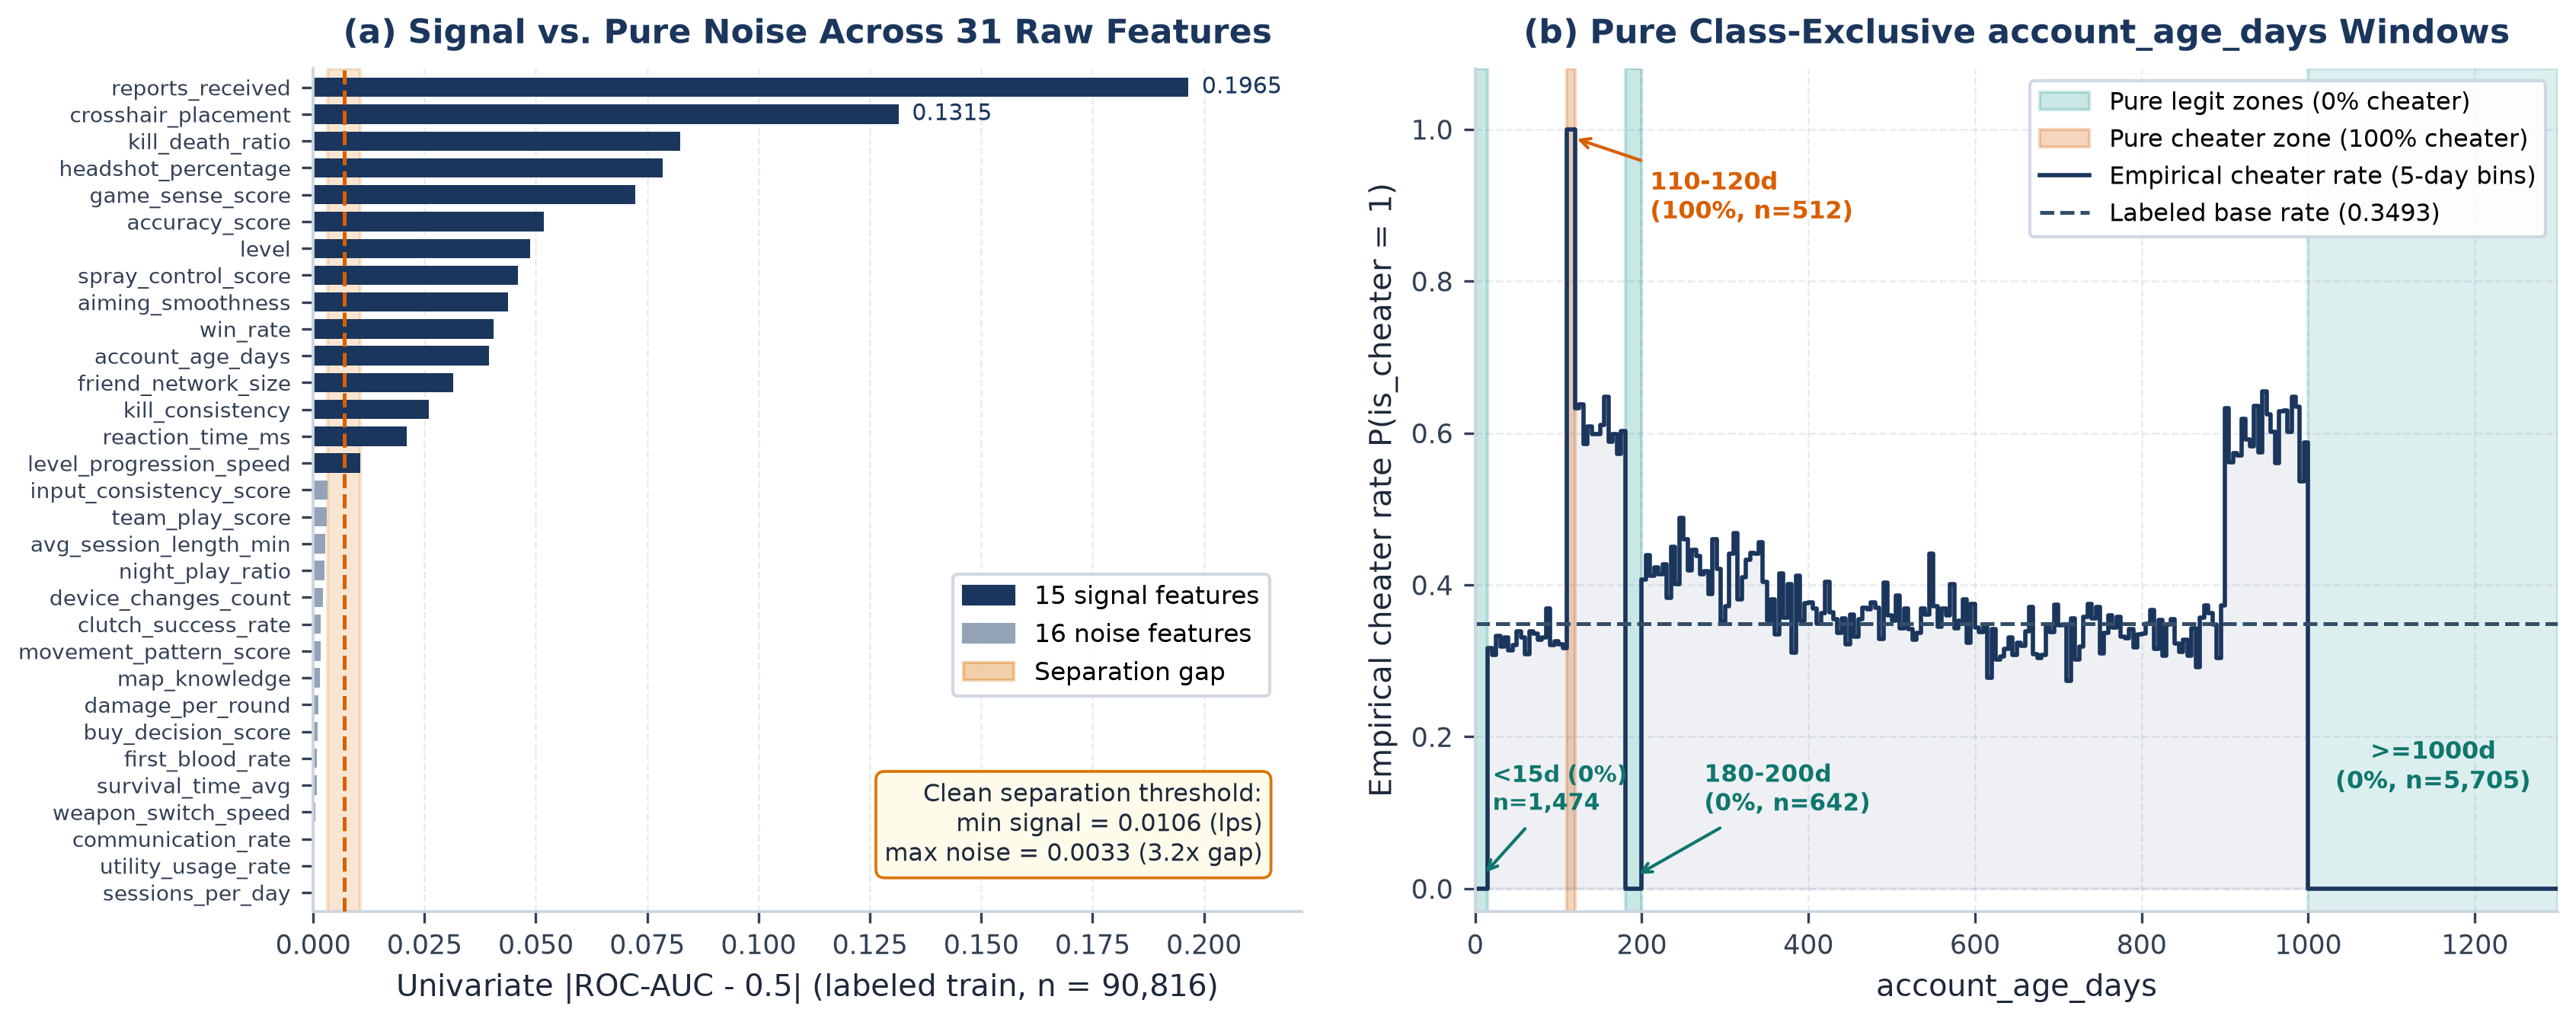
\includegraphics[width=0.98\textwidth]{figures/t1/fig_t1_signal_and_zones.png}
  \caption{ผลการวิเคราะห์ EDA ของ Task 1: (a) ค่า $|\text{ROC-AUC} - 0.5|$ แสดงการแยกขาด $3.2\times$ ระหว่าง $15$ ฟีเจอร์สัญญาณ ($\ge 0.0106$) และ $16$ ฟีเจอร์รบกวน ($\le 0.0033$); (b) หน้าต่าง \feat{account\_age\_days} ที่เป็นคลาสเดียว $100\%$ ได้แก่ $<15$ วัน ($0\%$, $n=1,474$), $110$--$120$ วัน ($100\%$, $n=512$), $180$--$200$ วัน ($0\%$, $n=642$) และ $\ge 1000$ วัน ($0\%$, $n=5,705$)}
  \label{fig:t1_signal_zones}
\end{figure}

\begin{figure}[htbp]
  \centering
  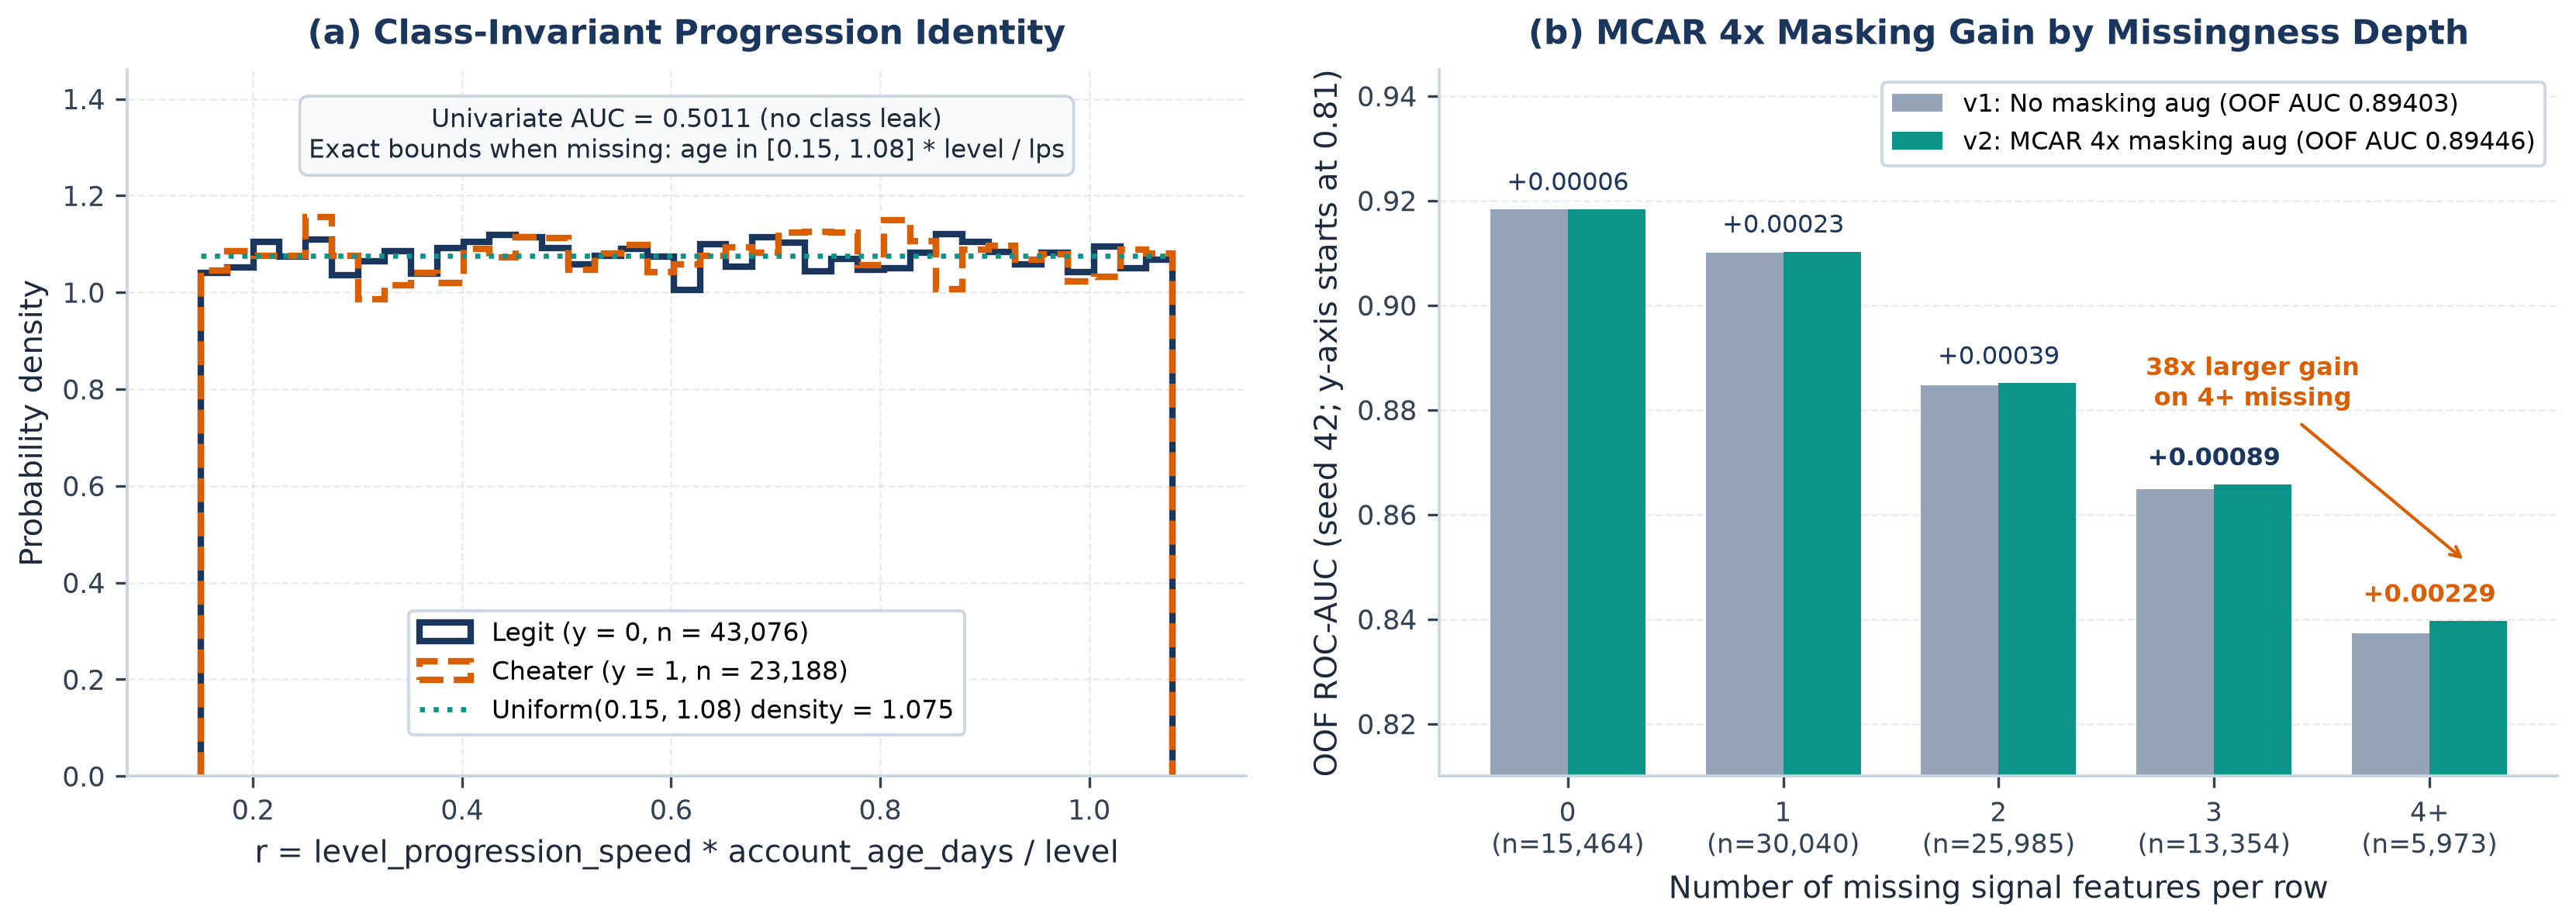
\includegraphics[width=0.98\textwidth]{figures/t1/fig_t1_lps_identity.png}
  \caption{(a) การแจกแจงแบบสม่ำเสมอ $U(0.15, 1.08)$ ของอัตราส่วน $r = \mathrm{lps} \times \mathrm{age} / \mathrm{level}$ (ระหว่าง \feat{level\_progression\_speed}, \feat{account\_age\_days} และ \feat{level}) ทั้งสองคลาส ($\text{AUC} = 0.5011$); (b) ผลต่าง OOF ROC-AUC ระหว่างรอบที่ 1 (\feat{v1}, ไม่ใช้ Masking, $0.89403$) และรอบที่ 2 (\feat{v2}, MCAR 4x Masking, $0.89446$) แยกตามจำนวนฟีเจอร์สัญญาณที่สูญหายต่อแถว โดยแถวที่หาย $4+$ คอลัมน์ได้กำไร $+0.00229$ (มากกว่าแถวที่ข้อมูลครบ $38\times$)}
  \label{fig:t1_lps_identity}
\end{figure}

\begin{insightbox}[สรุปโครงสร้างข้อมูลและขอบเขตความเป็นไปได้ของ Task 1]
ความสามารถในการจำแนกของ Task 1 ถูกขับเคลื่อนด้วยสองส่วนประกอบที่ชัดเจน: (1) ขอบเขต \textbf{Class-Exclusive Zones} ($34.2\%$ ของข้อมูลมีป้ายกำกับ) ที่โมเดลต้นไม้ตัดสินใจสามารถแยกแยะได้เกือบสมบูรณ์ และ (2) แกนกลางซ้อนทับ \textbf{Overlapping Core} ($65.8\%$ ของข้อมูล, $\text{Core AUC} \approx 0.773$--$0.774$) ซึ่งผลต่างระหว่างคลาสมาจากความน่าจะเป็นของจำนวนรายงาน/เพื่อน และค่าเฉลี่ยทักษะแบบมีนัยสำคัญแต่ซ้อนทับกันสูง ดังนั้นการเพิ่มประสิทธิภาพจึงต้องมุ่งไปที่การกู้คืนตำแหน่งโซนเมื่อข้อมูลสูญหายและการรักษาความแม่นยำในแถวที่ไม่สมบูรณ์
\end{insightbox}

\subsubsection{\texorpdfstring{การเตรียมข้อมูล Feature Engineering (fe\_v2) และ MCAR Masking Augmentation}{การเตรียมข้อมูล Feature Engineering (fe\_v2) และ MCAR Masking Augmentation}}

กระบวนการสร้างฟีเจอร์ถูกพัฒนาต่อยอดจากชุดพื้นฐาน \feat{fe\_baseline} ($44$ ฟีเจอร์) ซึ่งประกอบด้วย $15$ ฟีเจอร์สัญญาณ, $5$ ตัวบ่งชี้ค่าสูญหาย (\feat{na\_reports\_received}, \feat{na\_friend\_network\_size}, \feat{na\_account\_age\_days}, \feat{na\_crosshair\_placement}, \feat{na\_level}) กับ \feat{n\_missing}, ขอบเขตเชิงกำหนดจากเอกลักษณ์ \feat{lps} (\feat{age\_lo}, \feat{age\_hi}, \feat{age\_filled}, \feat{lv\_lo}, \feat{lv\_hi}, \feat{lvl\_filled}, \feat{r\_hat}), แฟล็กโซนพื้นฐาน (\feat{zone\_cheat}, \feat{zone\_legit}), การแปลง \texttt{log1p} $4$ ตัวแปร, สัดส่วนต่อ $100$ วันและสัดส่วนทักษะ (\feat{kd\_x\_hs}, \feat{acc\_x\_cross}, \feat{skill\_z\_sum}, \feat{skill\_z\_std}), ความถี่เชิงประจักษ์ (\feat{freq\_reports}, \feat{freq\_friends}) และ \feat{age\_segment}

ในเวอร์ชัน \feat{fe\_v2} ($56$ ฟีเจอร์, เพิ่ม $+12$ ฟีเจอร์จาก \feat{fe\_zone\_post}) เราแก้ปัญหาเมื่อ \feat{account\_age\_days} สูญหาย ($14.4\%$ ในชุดฝึกสอน) หรือ \feat{level} สูญหาย ($7.1\%$) ซึ่งค่ากลางเรขาคณิตแบบเดิมไม่สามารถบอกความน่าจะเป็นของการตกอยู่ในช่วงหน้าต่างแคบเช่น $110$--$120$ วัน หรือ $180$--$200$ วันได้ โดยใช้ \textbf{Exact Bayesian Zone Posteriors} บนกริดละเอียด $1$ วันสำหรับอายุบัญชี ($g_A \in \{0.5, 1.5, \dots, 1499.5\}$) และกริด $0.1$ หน่วยสำหรับเลเวล ($g_L \in [25.05, 99.95]$)

จากเอกลักษณ์ $\mathrm{lps} = \frac{\mathrm{level} \cdot r}{\mathrm{age}}$ เมื่อ $r \sim U(0.15, 1.08)$ ความหนาแน่นความน่าจะเป็นแบบมีเงื่อนไขของค่าที่สังเกตได้คือ Jacobian $|\partial r / \partial \mathrm{lps}| = \mathrm{age}/\mathrm{level}$ ดังนั้นเมื่อ \feat{account\_age\_days} สูญหายแต่ทราบ $(\mathrm{level}, \mathrm{lps})$ และเมื่อ \feat{level} สูญหายแต่ทราบ $(\mathrm{age}, \mathrm{lps})$ ความน่าจะเป็นภายหลังแบบไม่ใช้ป้ายกำกับ (Label-Free Posterior) คือ:
\begin{align}
P(\text{age} \mid \text{lps}, \text{level}) &\propto \text{prior}(\text{age}) \cdot \text{age} \cdot \mathbf{1}\!\left[\frac{\text{lps}\cdot\text{age}}{\text{level}} \in [0.15, 1.08]\right] \label{eq:t1_post_age}\\
P(\text{level} \mid \text{lps}, \text{age}) &\propto \text{prior}(\text{level}) \cdot \frac{1}{\text{level}} \cdot \mathbf{1}\!\left[\frac{\text{lps}\cdot\text{age}}{\text{level}} \in [0.15, 1.08]\right] \label{eq:t1_post_lvl}
\end{align}
ค่าแจกแจงก่อนหน้าเชิงประจักษ์ ($\text{prior}(\text{age})$ และ $\text{prior}(\text{level})$ พร้อมตัวปรับเรียบ Laplace $+0.5$) ถูกคำนวณจากแถวฝึกสอนเท่านั้น ($90,816$ แถวมีป้ายกำกับ $+ 13,184$ แถวไม่มีป้ายกำกับ รวม $104,000$ แถว) โดยไม่แตะต้องข้อมูลทดสอบ จากสมการ~\eqref{eq:t1_post_age}--\eqref{eq:t1_post_lvl} เราสกัดฟีเจอร์ใหม่ $12$ ตัว ได้แก่ ความน่าจะเป็นใน $6$ ช่วงอายุ (\feat{pa\_cheat\_110\_120}, \feat{pa\_legit\_lt15}, \feat{pa\_legit\_180\_200}, \feat{pa\_legit\_ge1000}, \feat{pa\_young\_lt110}, \feat{pa\_mid\_120\_180}), ค่าคาดหวัง \feat{age\_post\_mean}, ความน่าจะเป็นใน $2$ ช่วงเลเวล (\feat{pl\_cheat\_lt28}, \feat{pl\_legit\_gt96}), ค่าคาดหวัง \feat{lvl\_post\_mean} และตัวแปรรวมความเสี่ยงโซน \feat{p\_cheat\_zone}, \feat{p\_legit\_zone} การทดลอง \feat{exp03} ยืนยันว่า \feat{fe\_v2} เพิ่ม 3-seed OOF AUC จาก $0.89244$ เป็น $0.89315$ ($+0.00071$) และ Nested Macro-$F_2$ จาก $0.78006$ เป็น $0.78108$ ($+0.00102$)

ต่อมาการวิเคราะห์ความผิดพลาดเผยว่าความสามารถในการจำแนกลดฮวบในแถวที่มีค่าสูญหายมาก (OOF AUC ลดจาก $0.91828$ เมื่อขาด $0$ ฟีเจอร์ เหลือ $0.83736$ เมื่อขาด $4+$ ฟีเจอร์; โดยเฉพาะแถวที่ขาด \feat{reports\_received}, \feat{friend\_network\_size}, \feat{account\_age\_days} หรือ \feat{crosshair\_placement} มี AUC เพียง $0.854$--$0.863$) เนื่องจากแต่ละฟอลด์มีแถวที่ขาดฟีเจอร์สำคัญเพียงราว $16,000$ แถวจาก $72,000$ แถว เพื่อใช้ประโยชน์จากสมบัติ MCAR เราจึงพัฒนาเทคนิค \textbf{MCAR 4x Masking Augmentation} (\feat{exp16}, \feat{final\_v2.py}):
\begin{enumerate}
  \item ภายในแต่ละฟอลด์ฝึกสอน หลังแยกชุด Validation ย่อย $10\%$ สำหรับ Early Stopping ออกไปแล้ว เราสร้างสำเนาของข้อมูลฝึกสอนจำนวน $NC = 4$ ชุด
  \item ในแต่ละสำเนา สุ่มปิดบังค่าใน $15$ ฟีเจอร์สัญญาณเป็น \texttt{NaN} ด้วยความน่าจะเป็นเท่ากับอัตราการสูญหายเชิงประจักษ์ของแต่ละคอลัมน์ ($\text{RATE} = 1.0$)
  \item \textbf{คำนวณ \feat{fe\_v2} ใหม่ทั้งหมดบนข้อมูลที่ถูกปิดบัง} เพื่อให้ค่าบ่งชี้ \feat{na\_*}, \feat{n\_missing}, ขอบเขต \feat{lps} และ Bayesian Zone Posteriors สอดคล้องกับสถานะค่าสูญหายที่เกิดขึ้นจริง ส่วนชุด Early Stopping, Validation Fold และ Test Set จะไม่ถูกปรับแต่งใดๆ ทั้งสิ้น
\end{enumerate}
ตาราง~\ref{tab:t1_mcar_depth} และรูปที่~\ref{fig:t1_lps_identity}b แสดงผลเปรียบเทียบแบบแบ่งชั้นความลึกของค่าสูญหายระหว่าง \feat{v1\_best\_oof.npy} ($0.89403$) และ \feat{best\_oof.npy} ($0.89446$) บน seed 42 พบว่าแถวที่ข้อมูลครบได้กำไรเพียง $+0.00006$ ขณะที่แถวซึ่งขาด $4+$ ฟีเจอร์ได้กำไรถึง $+0.00229$ (สูงกว่า $38\times$) ยืนยันว่าการจำลองความไม่สมบูรณ์ของข้อมูลช่วยให้โมเดลเรียนรู้โครงสร้างความน่าจะเป็นแบบ Marginals ได้แม่นยำขึ้นมาก

\begin{table}[htbp]
  \centering
  \small
  \setlength{\tabcolsep}{6pt}
  \caption{การเพิ่มขึ้นของ OOF ROC-AUC (seed 42) จาก MCAR 4x Masking Augmentation จำแนกตามจำนวนฟีเจอร์สัญญาณที่สูญหายต่อแถว}
  \label{tab:t1_mcar_depth}
  \begin{tabular}{@{}p{4.8cm}rrrr@{}}
    \toprule
    \textbf{จำนวนฟีเจอร์สัญญาณที่สูญหาย} & \shortstack[r]{\textbf{จำนวนแถว}\\\textbf{($n$)}} & \shortstack[r]{\textbf{Round 1}\\\textbf{(No Aug)}} & \shortstack[r]{\textbf{Round 2}\\\textbf{(MCAR 4x)}} & \shortstack[r]{\textbf{ผลต่าง AUC}\\\textbf{($\Delta$)}} \\
    \midrule
    $0$ คอลัมน์ (ข้อมูลครบ) & $15,464$ & $0.91828$ & $0.91834$ & $+0.00006$ \\
    $1$ คอลัมน์ & $30,040$ & $0.91002$ & $0.91025$ & $+0.00023$ \\
    $2$ คอลัมน์ & $25,985$ & $0.88471$ & $0.88510$ & $+0.00039$ \\
    $3$ คอลัมน์ & $13,354$ & $0.86486$ & $0.86575$ & $+0.00089$ \\
    $4+$ คอลัมน์ & $5,973$ & $0.83736$ & $0.83965$ & $\mathbf{+0.00229}$ ($38\times$) \\
    \midrule
    \textbf{รวมทั้งชุดข้อมูล OOF} & $\mathbf{90,816}$ & $\mathbf{0.89403}$ & $\mathbf{0.89446}$ & $\mathbf{+0.00043}$ \\
    \bottomrule
  \end{tabular}
\end{table}

\subsubsection{การออกแบบโมเดล Diversity Rank Blend และเหตุผลเชิงวิศวกรรม}

จากการทดสอบตระกูลโมเดลที่หลากหลายใน \feat{t1/research/} และ \feat{t1/research/blind\_sonnet/} พบว่า \textbf{LightGBM} (\feat{final\_v2}: Optuna baseline hyperparameters ได้แก่ \feat{num\_leaves} $= 39$, \feat{min\_child\_samples} $= 8$, \feat{subsample} $= 0.814$, \feat{colsample\_bytree} $= 0.455$, \feat{reg\_lambda} $= 4.01$, \feat{max\_bin} $= 511$, \feat{learning\_rate} $= 0.02$, Early Stopping $200$ รอบบนชุดแยก $10\%$, เฉลี่ย $3$ bags $\times$ $5$ folds $\times$ $3$ seeds รวม $45$ โมเดล) เอาชนะสถาปัตยกรรมทางเลือกทุกชนิดอย่างขาดลอย:
\begin{itemize}
  \item \textbf{Neural Network (MLP)}: โมเดล PyTorch MLP พร้อม Piecewise-Linear Encoding (\feat{PLE16 3x256}, \feat{exp09}, 3 seeds) ทำ OOF AUC ได้เพียง $0.88548$ และ Binary-$F_2$ $0.83473$ (ส่วน MLP $128$-$64$ ใน \feat{blind\_sonnet} ได้ AUC $0.8468$, Binary-$F_2$ $0.8051$) เพราะชั้นเชิงเส้นและฟังก์ชันกระตุ้นแบบเรียบไม่เหมาะกับการจับขอบเขตสี่เหลี่ยมที่ตัดขาดแบบขั้นบันได
  \item \textbf{Mixture Naive Bayes}: แม้ใช้ Mixture NB แบบ Marginalize ค่า \texttt{NaN} ด้วย EM ($K=(6,3)$ ใน \feat{exp04}/\feat{exp07}) ก็ได้ AUC สูงสุดเพียง $0.87451$ (seed 42) และ $0.86957$ เฉลี่ย 3 seeds (Binary-$F_2$ $0.82083$) ส่วน Gaussian NB มาตรฐานได้เพียง $0.7304$ AUC / $0.7513$ Binary-$F_2$ เนื่องจากสหสัมพันธ์ภายในคลาสระหว่างกลุ่มทักษะ ($\rho \approx 0.3$) ละเมิดสมมติฐานความเป็นอิสระเชิงเงื่อนไข
  \item \textbf{ExtraTrees, SVM และ kNN}: ExtraTrees ($200$ ต้น, \feat{leaf=10}) ได้ AUC $0.8611$ / Binary-$F_2$ $0.8110$ เพราะการสุ่มจุดแบ่งลดความคมของขอบเขตโซน; Linear SVM บน Spline Basis ($8$ knots) ได้ $0.8391$ / $0.8058$; LinearSVC ($0.7663$ / $0.7651$), RBF SVC ($10\text{k}$ subsample, $0.7646$ / $0.7556$) และ Nystroem+SGD ($0.7698$ / $0.7561$) อ่อนกำลังจากขอบเขตไม่เป็นเชิงเส้นและการประมาณเคอร์เนล; ส่วน kNN ($k=100$, $20\text{k}$ subsample) ได้เพียง $0.6893$ AUC / $0.7284$ Binary-$F_2$ (ไม่ดีกว่าการทำนายบวกทั้งหมดที่ $\sim 0.729$)
\end{itemize}

แม้ LightGBM จะเป็นแกนหลัก แต่การผสานความหลากหลายเชิงสถาปัตยกรรม (Architectural Diversity) ในสัดส่วนที่พอเหมาะช่วยลดความแปรปรวนบริเวณหางล่างของการจัดอันดับที่ $\text{Recall} \approx 97\%$ จึงเกิดเป็นสูตร \textbf{3-Component Diversity Blend}:
\begin{equation}
S_{\text{blend}} = 0.70 \cdot E_{\text{final\_v2}} + 0.20 \cdot E_{\text{stack\_lr}} + 0.10 \cdot E_{\text{gbm\_pipe}}
\label{eq:t1_blend}
\end{equation}
โดยองค์ประกอบทั้งสามได้แก่ (1) \feat{final\_v2} ($70\%$): ความน่าจะเป็นเฉลี่ย 3 seeds ของ LightGBM พร้อม \feat{fe\_v2} และ MCAR 4x Masking; (2) \feat{blind\_sonnet/stack\_lr} ($20\%$): Meta-learner แบบ Logistic Regression ที่ซ้อน Logits ของโมเดลต่างสายพันธุ์ $4$ ตัว (\feat{gbm\_eng\_sig} น้ำหนัก $+1.23$, \feat{extra\_trees}, \feat{nn\_mlp} และ \feat{svm\_spline} น้ำหนัก $-0.51$, ซึ่งตัวมันเองได้ AUC $0.8928$, Binary-$F_2$ $0.8383$); และ (3) \feat{t1\_pipeline} ($10\%$): โครงสร้าง Optuna 3-GBM ผสมบน \feat{fe\_baseline} ($0.1834\,\text{XGBoost} + 0.4848\,\text{LightGBM} + 0.3318\,\text{CatBoost}$ ที่ใช้ categorical binning)

\begin{decisionbox}[การปรับรหัสตามกติกา TA 16 Nov: จาก Test-Rank Quantile Cut สู่ Clean OOF ECDF + Fixed Threshold (\texttt{t1\_clean\_fixedthr.py})]
ในเวอร์ชัน \feat{sub\_v20a} มีการใช้ Rank Normalization บนชุดทดสอบและตัดจุดแบ่งตามสัดส่วนทดสอบบนสุด $60\%$ ซึ่งเข้าข่ายการพึ่งพาข้อมูลข้ามแถวในชุดทดสอบ (Test-Batch Coupling) หลังการตรวจสอบความสอดคล้องกับกติกาวันที่ 16 พฤศจิกายน ทีมจึงปรับแก้เป็นสคริปต์ \feat{t1/code/t1\_clean\_fixedthr.py} โดยคงโมเดลและน้ำหนัก $(0.70, 0.20, 0.10)$ เดิมทั้งหมด แต่เปลี่ยนฟังก์ชัน $E_m(\cdot)$ ในสมการ~\eqref{eq:t1_blend} ให้เป็น \textbf{Train-Only OOF ECDF Mapping} ($E_m(v) = \frac{1}{N_{\text{oof}}} \sum_{i=1}^{N_{\text{oof}}} \mathbf{1}[\text{oof}_{m,i} \le v]$) เพื่อแปลงคะแนนทำนายของแต่ละแถวทดสอบโดยอ้างอิงกับแจกแจง OOF ที่แช่แข็งไว้เท่านั้น ไม่มีการเปรียบเทียบระหว่างแถวทดสอบ

จากนั้นจึงหาจุดตัดคงที่บน OOF Blend ($\text{OOF ROC-AUC} = 0.89499$) ได้จุดตัดเหมาะสมสำหรับ Binary-$F_2$ คือ $\text{thr} = 0.3769$ ซึ่งให้ \textbf{OOF Binary-$F_2 = 0.84007$} ที่อัตราบวก OOF $62.40\%$ (เทียบกับ $0.83717$ หากตัดที่ $60\%$ OOF) เมื่อนำจุดตัดคงที่ $\text{thr} = 0.3769$ ไปใช้กับชุดทดสอบโดยตรง พบว่าสัดส่วนทำนายบวกบนชุดทดสอบลดลงเหลือ $\mathbf{59.33\%}$ ($15,359$ จาก $25,889$ แถว) เหตุผลเชิงกายภาพได้รับการยืนยันจากการค้นพบใน \feat{round9\_sonnet}: ชุดทดสอบมีค่าสูญหายน้อยกว่าชุดฝึกสอนอย่างชัดเจน (ค่าเฉลี่ย \texttt{NaN} ต่อแถว $2.48$ เทียบกับ $3.71$; Adversarial AUC Train-vs-Test $= 0.90$ ซึ่งขับเคลื่อนจากอัตราการสูญหายเพียงอย่างเดียว โดย \feat{account\_age\_days} ลดการหายจาก $14.4\% \rightarrow 0.6\%$, \feat{friend\_network\_size} $22\% \rightarrow 4.7\%$, \feat{aiming\_smoothness} $21\% \rightarrow 2.1\%$, \feat{level} $7.1\% \rightarrow 1.5\%$ ขณะที่บางคอลัมน์ทักษะหายมากขึ้นเล็กน้อย เช่น \feat{headshot\_percentage} $2.7\% \rightarrow 14.1\%$) เมื่อฟีเจอร์โครงสร้างหลักถูกสังเกตครบถ้วนขึ้น โมเดลจึงประเมินผู้เล่นปกติได้เด็ดขาดกว่าเดิมและผลักคะแนนลงต่ำกว่า $0.3769$ อย่างสุจริตโดยไม่บิดเบือนตามสถิติชุดทดสอบ
\end{decisionbox}

\subsubsection{กลยุทธ์การวัดผล ลำดับการทดลอง และผลลัพธ์สุดท้าย}

การวัดผลทั้งหมดดำเนินภายใต้กรอบ 5-fold StratifiedKFold ซ้ำ $3$ seeds ($42, 7, 2024$) โดยแยก $10\%$ ภายในแต่ละ Training Fold เพื่อ Early Stopping และวัดคะแนน $F_2$ ด้วยวิธี \textbf{Nested Threshold Evaluation} (หาจุดตัดที่เหมาะสมบน OOF ของ $4$ ฟอลด์ฝึกแล้วนำไปวัดบนฟอลด์ที่ $5$) เพื่อขจัดการเลือกจุดตัดแบบมองย้อนหลัง จาก \feat{exp21} พบว่าการวัดแบบ In-sample ($0.9216$ AUC / $0.8188$ Macro-$F_2$ / $0.8535$ Binary-$F_2$) และชุด Holdout $10\%$ เดี่ยว ($0.8971$ / $0.7885$ / $0.8444$) ล้วนสูงเกินจริง เมื่อเทียบกับ 3-seed Nested OOF ที่เชื่อถือได้ของ \feat{final\_v2} ($0.89482$ AUC / $0.78279$ Macro-$F_2$ / $0.83911$ Binary-$F_2$)

ตาราง~\ref{tab:t1_progression} สรุปลำดับพัฒนาการของโมเดลตั้งแต่ Baseline จนถึง Clean ECDF Blend ขั้นสุดท้าย พร้อมหลักฐานสำคัญบน Public Leaderboard สองรายการ:
\begin{enumerate}
  \item \textbf{Isolated LB Probe (\feat{sub\_v10d} $\rightarrow$ \feat{probe\_v10e})}: การปรับเฉพาะจุดตัดของ Task 1 จากสมมติฐาน Macro-$F_2$ ($41\%$ positive) เป็นจุดตัด Binary-$F_2$ ($63\%$ positive) โดยคงโมเดลของ Task 2--5 ไว้เหมือนเดิม เพิ่มคะแนนรวม LB จาก $0.66614$ เป็น $\mathbf{0.67890}$ ($\mathbf{+0.01276}$ หรือ $+0.0128$ LB) ยืนยันว่าเกณฑ์ประเมินบน LB คือ Binary-$F_2$
  \item \textbf{Diversity Rank Blend (\feat{sub\_v18a} $\rightarrow$ \feat{sub\_v20a})}: การผสมผสาน $3$ ตระกูลโมเดลเพิ่มคะแนนรวม LB จาก $0.71999$ เป็น $0.72016$ ($+0.00017$ LB) ก่อนถูกแปลงเป็นระบบ \feat{t1\_clean\_fixedthr.py} ที่ปลอด Test Leakage โดยสมบูรณ์
\end{enumerate}

\begin{table}[htbp]
  \centering
  \footnotesize
  \setlength{\tabcolsep}{3.5pt}
  \caption{ลำดับพัฒนาการของโมเดล Task 1 บน 5-fold StratifiedKFold (3 seeds: $42, 7, 2024$) และ Clean ECDF Blend}
  \label{tab:t1_progression}
  \begin{tabularx}{\textwidth}{@{} >{\raggedright\arraybackslash}p{4.5cm} r r r r >{\raggedright\arraybackslash}X @{}}
    \toprule
    \textbf{ขั้นตอนการทดลอง / โมเดล} & \shortstack[r]{\textbf{OOF}\\\textbf{AUC}} & \shortstack[r]{\textbf{Macro-$F_2$}\\\textbf{(Nested)}} & \shortstack[r]{\textbf{Bin-$F_2$}\\\textbf{(OOF-opt)}} & \shortstack[r]{\textbf{Bin-$F_2$}\\\textbf{(Nested)}} & \textbf{หมายเหตุสำคัญ} \\
    \midrule
    Baseline Single Models (Cat / XGB / LGB) & $.8912$--$.8919$ & $.7779$--$.7784$ & $.8373$--$.8377$ & $.8370$--$.8375$ & Seed 42 (Pipeline เดิม) \\
    Baseline 3-Model Rank Blend (\feat{oof\_blend}) & $0.89248$ & $0.77987$ & $0.83834$ & $0.83819$ & Seed 42 อ้างอิงเริ่มต้น \\
    \feat{exp02}: LGB \feat{fe\_baseline} ($44$ feats, lr $0.05$) & $0.89244$ & $0.78006$ & $0.83776$ & $0.83749$ & ตัด $16$ Noise Columns \\
    \feat{exp03}: + \feat{fe\_v2} Bayesian Zone Posteriors ($56$ feats) & $0.89315$ & $0.78108$ & $0.83840$ & $0.83798$ & เพิ่ม $+0.00102$ F2m (ทุก seed) \\
    \feat{exp05}: \feat{fe\_v2} + Learning Rate $0.02$ & $0.89374$ & $0.78151$ & $0.83890$ & $0.83858$ & ลด LR ช่วยขอบเขตละเอียด \\
    \feat{final} (Round 1): + $3$ bags/fold (No Aug) & $0.89412$ & $0.78184$ & $0.83904$ & $0.83877$ & เฉลี่ย 3 seeds $\pm 0.00008$ AUC \\
    \feat{final\_v2} (Round 2): + MCAR 4x Masking (mean) & $0.89453$ & $0.78201$ & $0.83938$ & $0.83911$ & AUC $+0.00041$ เหนือ Round 1 \\
    \feat{final\_v2} 3-Seed Averaged OOF (\feat{avg3\_oof}) & $0.89482$ & $0.78279$ & $0.83948$ & $0.83911$ & $45$ โมเดล (5f $\times$ 3s $\times$ 3b) \\
    \midrule
    \textbf{Final Clean ECDF Blend (\feat{t1\_clean\_fixedthr})} & $\mathbf{0.89499}$ & --- & $\mathbf{0.84007}$ & --- & \textbf{Fixed $\text{thr}=0.3769$; Test $59.33\%$ ($15,359$ แถว); OOF F2m $0.7833$} \\
    \bottomrule
  \end{tabularx}
\end{table}

รูปที่~\ref{fig:t1_f2_operating_point} แสดงความสัมพันธ์ของค่า OOF Binary-$F_2$ เทียบกับ Macro-$F_2$ ตลอดช่วงอัตราทำนายบวก $25\%$--$85\%$ บน Clean ECDF Blend ซึ่งเห็นจุดสมดุลของ Macro-$F_2$ ($\sim 40.7\%$--$41.3\%$) เทียบกับจุดสูงสุดของ Binary-$F_2$ ($62.40\%$ OOF ที่ $0.84007$), ก้าวกระโดด $+0.0128$ LB ของ probe และจุดทำงานจริงบนชุดทดสอบที่ $59.33\%$

\begin{figure}[htbp]
  \centering
  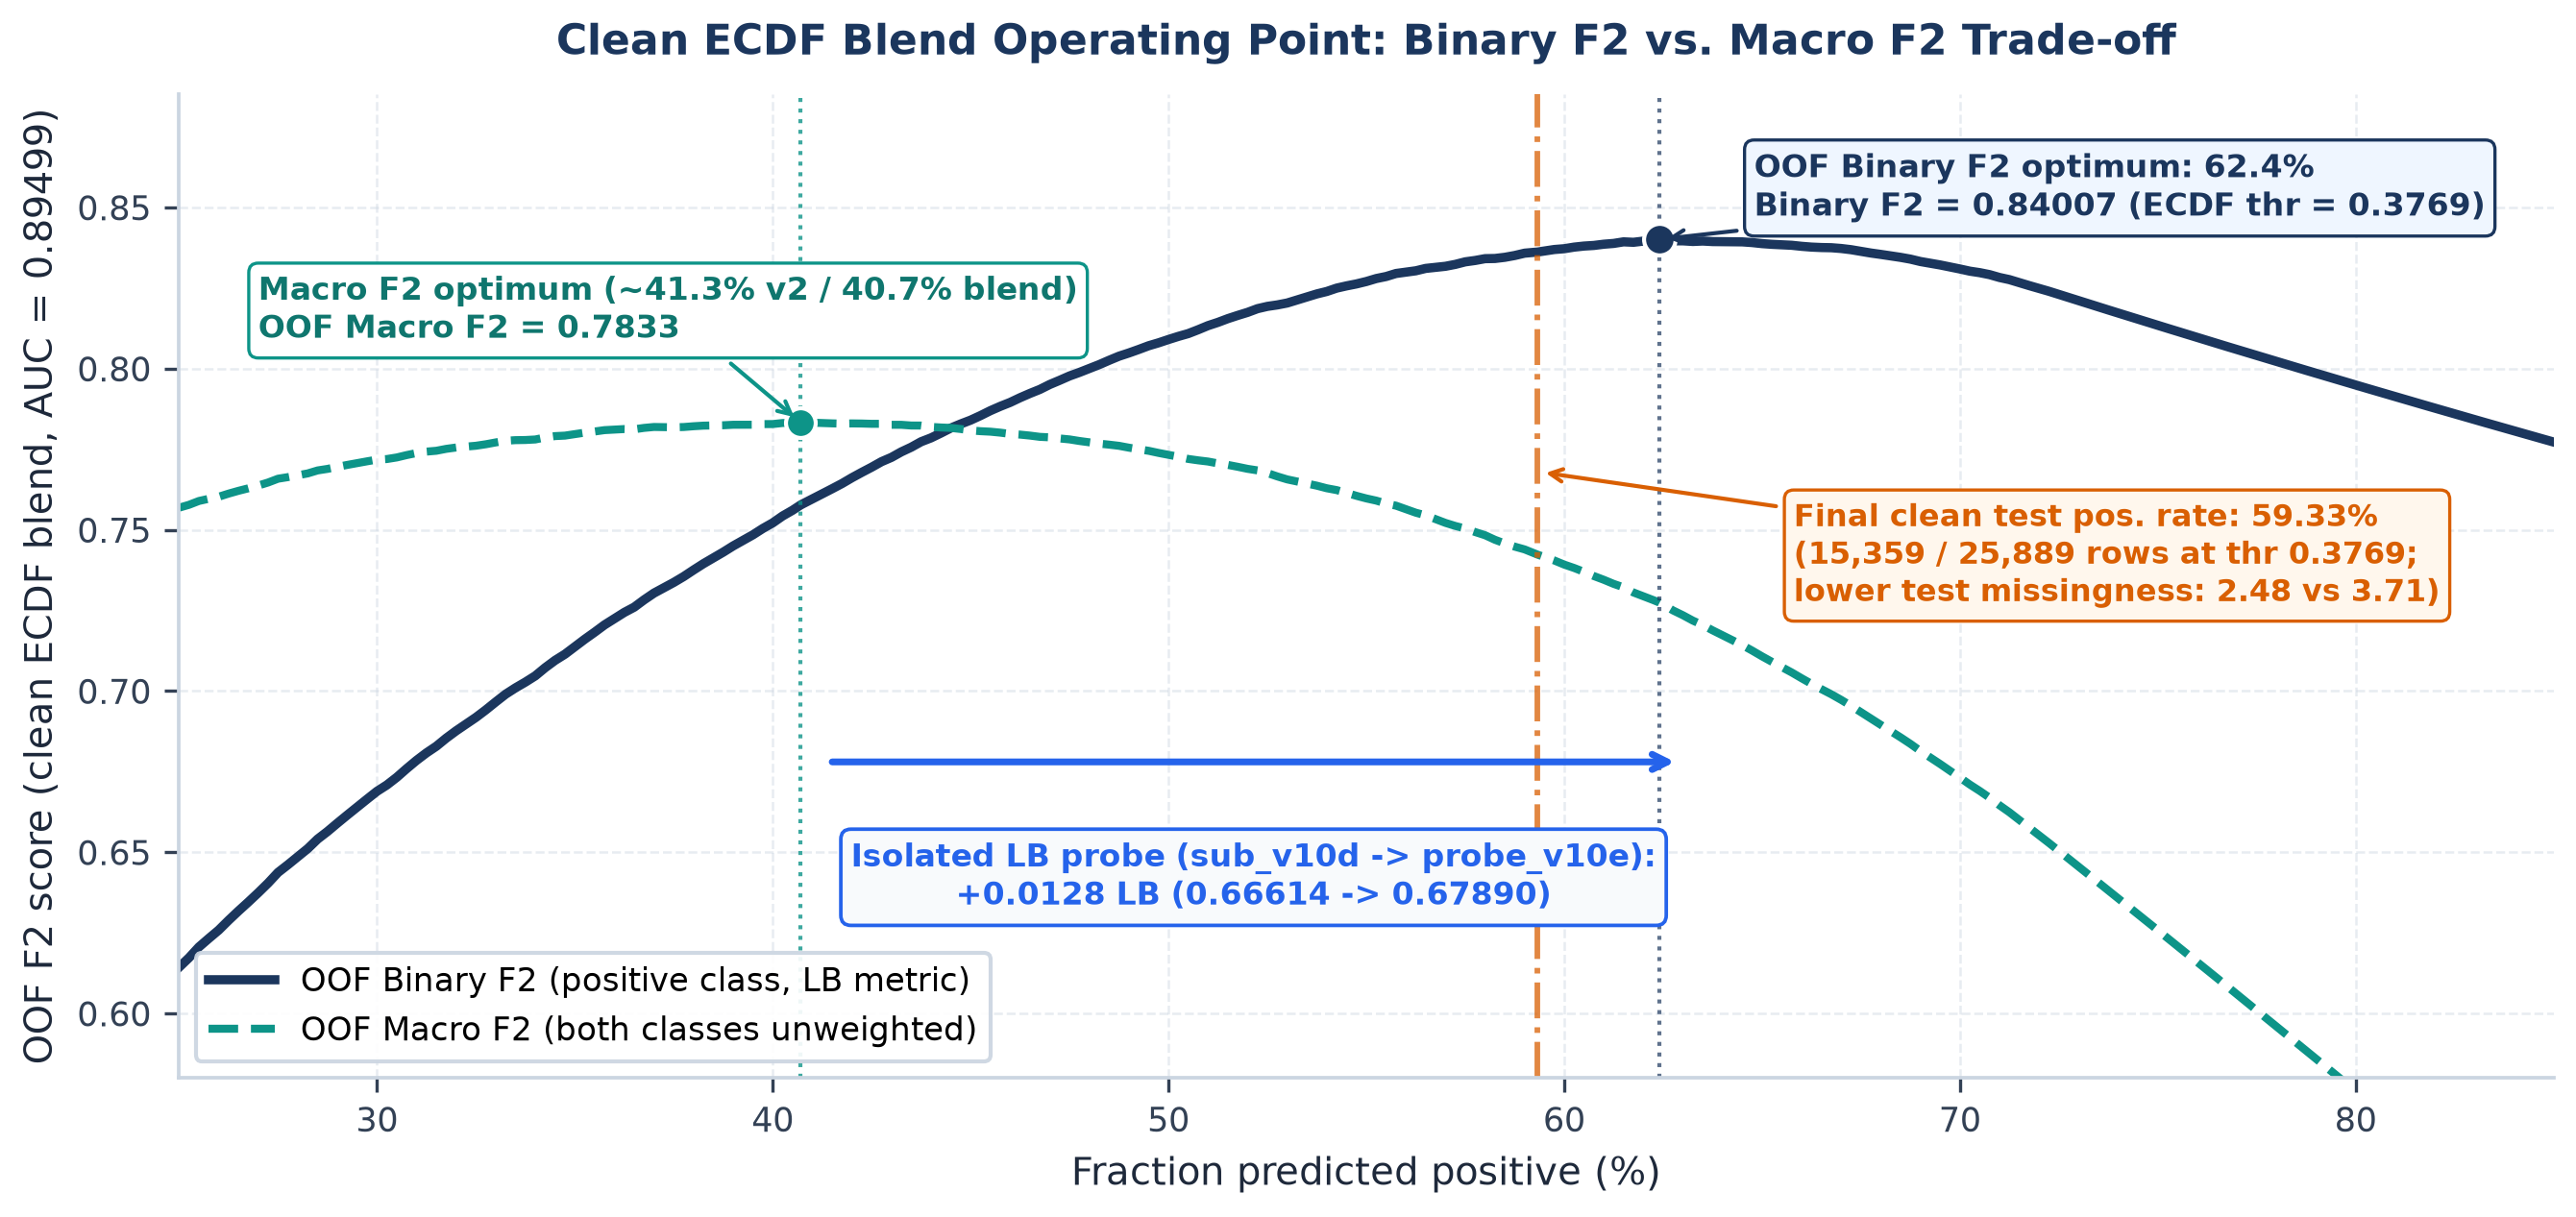
\includegraphics[width=0.96\textwidth]{figures/t1/fig_t1_f2_operating_point.png}
  \caption{เส้นโค้งจุดทำงานของ Clean ECDF Blend ($\text{OOF AUC} = 0.89499$): เปรียบเทียบจุดสูงสุดของ Macro-$F_2$ ($\sim 40.7\%$--$41.3\%$, $0.7833$) กับ Binary-$F_2$ ($62.40\%$ OOF ที่ $\text{thr} = 0.3769$, $0.84007$), การยืนยันจาก LB Probe (\feat{sub\_v10d} $\rightarrow$ \feat{probe\_v10e}: $0.66614 \rightarrow 0.67890$, $+0.0128$ LB) และสัดส่วนบวกบนชุดทดสอบ $59.33\%$ ($15,359 / 25,889$ แถว)}
  \label{fig:t1_f2_operating_point}
\end{figure}

\subsubsection{การวิเคราะห์พฤติกรรมโมเดล การทดลองที่ไม่ได้ผล และเพดานของข้อมูล}

ตลอด 8 รอบการวิจัยและรอบตรวจสอบความแปรปรวนเพิ่มเติม ทีมได้ทดสอบสมมติฐานจำนวนมากที่ไม่ประสบผลสำเร็จและถูกคัดออกอย่างมีวินัย เพื่อป้องกันความซับซ้อนเกินจำเป็นและไม่หลงเชื่อสัญญาณรบกวน (ผลต่าง Nested Score $< 0.001$) ดังสรุปในตาราง~\ref{tab:t1_failed}

\begin{table}[htbp]
  \centering
  \footnotesize
  \setlength{\tabcolsep}{4.5pt}
  \caption{สรุปการทดลองที่ไม่ช่วยเพิ่มประสิทธิภาพจริง (Failed / Rejected Experiments) และสาเหตุเชิงวิศวกรรม}
  \label{tab:t1_failed}
  \begin{tabular}{@{}p{4.3cm}p{4.1cm}p{6.6cm}@{}}
    \toprule
    \textbf{แนวคิด / การทดลอง} & \textbf{ผลลัพธ์ (CV / LB)} & \textbf{สาเหตุเชิงวิศวกรรมที่แท้จริง} \\
    \midrule
    ใส่กลับ $16$ Noise Features (\feat{exp02}) & AUC $0.89244 \rightarrow 0.89202$ ($-0.00042$) & สัมพันธ์กับสัญญาณเท่ากันทั้ง 2 คลาส จึงทำให้จุดตัดต้นไม้เจือจาง \\
    Hint \feat{game\_sense\_score}/\feat{accuracy\_score} และ $45$ Log-ratios (\feat{exp08}, $104$ feats) & F2m nested $0.78117$ / $0.78114$ vs $0.78108$ & ต้นไม้แบ่งแกนทักษะเกาส์เซียนได้ดีอยู่แล้ว อัตราส่วนเพิ่มเพียง noise \\
    Semi-supervised EM \& Pseudo-labeling $13\text{k}$ แถว (\feat{exp07/11/19}, \feat{v22a/b}) & AUC $0.86957 \rightarrow 0.86847$ (\feat{exp07}); F2m $-0.0006$ (\feat{exp11}); LB \feat{v21a} $0.76315 \rightarrow$ \feat{v22a} $0.76307$ / \feat{v22b} $0.76309$ & แถวไม่มีป้ายกำกับ $13,184$ แถวเป็น MCAR ในแจกแจงเดียวกับ $90\text{k}$ แถว; \feat{exp19} พิสูจน์ว่าแม้ใช้\textbf{ป้ายจริง}ก็ได้เพียง $+0.00098$ F2m ($0.78108$ vs $0.78010$) Pseudo-label จึงกู้ไม่ขึ้น \\
    Optuna Re-tuning บน \feat{fe\_v2} (\feat{exp10}, \feat{exp20}: 120 LGB / 50 XGB / 40 Cat) & Tune AUC เพิ่ม $+0.0007$ แต่ 3-seed CV ตก ($0.89315 \rightarrow 0.89276$) & Overfit ต่อ Split ปรับจูน; พารามิเตอร์ baseline (200 trials) อยู่ที่จุดอิ่มตัวแล้ว \\
    Cost-sensitive Weights (\feat{spw}=1.86/3/6), Focal Loss, \feat{pAUC\_hr} ES (\feat{exp05/22}) & \feat{spw=6} ทำ AUC พังเหลือ $0.85944$; \feat{spw=3}/Focal เพิ่ม binF2 แค่ $+0.0003$--$0.0005$ & การจัดอันดับ (AUC) + จุดตัดปลายทางให้ Bayes-optimal decision สำหรับ $F_2$ แล้ว ไม่จำเป็นต้องบิด Loss \\
    Label Denoising / Drop Hard Rows (\feat{exp23}: $2\%, 5\%, 10\%$) & ลบ $2\%/5\%/10\%$ ทำ AUC ตก $0.8922/0.8890/0.8821$, binF2 ตกเหลือ $0.82020$ & มีโอกาสเป็น Label flip เพียง $0.12\%$ แถวที่ทายยากคือ Core Bayes overlap; การลบทิ้งทำให้โมเดลมั่นใจเกินจริงตรงจุดตัด Recall สูง \\
    Label-free LGB Imputers (\feat{exp12}, \feat{fe\_v3}) & AUC $0.89306$, F2m $0.78105$ ($\le 0.78108$) & การเดาค่าหายจากคอลัมน์อื่นให้เพียงข้อมูลพร็อกซีที่ GBM เห็นอยู่แล้ว \\
    Nested OOF kNN Target Rate (\feat{exp14}, $k=25,100,400$) & AUC $0.8926/0.8924$, F2m $0.7799/0.7795$ & kNN เดี่ยวได้ AUC $0.795$ จึงเติมสัญญาณรบกวนมากกว่าข้อมูลใหม่ \\
    Hard Zone Overrides \& Per-Group Threshold/Isotonic (\feat{exp17}) & Force $31,055$ แถวได้ $+0.00001$ F2m; Per-group ได้ $0.78166$ (แย่ลง) & GBM ทายแถวในโซนบริสุทธิ์ถูก $100\%$ อยู่แล้ว; การแบ่งกลุ่มจูนจุดตัดเพิ่มความแปรปรวน \\
    Cross-fitted Linear Skill Logits (\feat{INSIGHTS.md b03}) & F2m $-0.00016$ / $-0.00059$, binF2 $-0.00006$ / $+0.00015$ & โมเดล GBM ดึง Mean Shift เชิงเส้นของกลุ่มทักษะออกไปใช้หมดแล้ว \\
    Test-shift Mask Augmentation (\feat{round9\_sonnet}) & binF2 $+0.00049$ ($0.83808 \rightarrow 0.83857$ บน fold 0--1) & ผลต่างระดับ noise ($< 0.003$) ไม่คุ้มค่ากับความเสี่ยงต่อ Overfitting \\
    \bottomrule
  \end{tabular}
\end{table}

\textbf{การพิสูจน์เพดานเชิงปริมาณของข้อมูล (Quantitative Data Ceiling)}: ใน \feat{exp18\_ceiling.py} ทีมได้ทดสอบ Learning Curve โดยฝึก LightGBM บน \feat{fe\_v2} ด้วยสัดส่วนข้อมูล $10\%$ ถึง $100\%$ ($\sim 7,265$ ถึง $72,652$ แถว) ผลลัพธ์ F2m เพิ่มจาก $0.7625 \rightarrow 0.7725 \rightarrow 0.7767 \rightarrow 0.7787 \rightarrow 0.7796 \rightarrow 0.7811$ เมื่อฟิตเส้นโค้งกฎกำลัง $s(n) = s_\infty - a n^{-b}$ ได้ค่าเส้นกำกับเมื่อมีข้อมูลไม่จำกัด (Asymptote) ที่ \textbf{AUC $= 0.8939$} และ \textbf{Macro-$F_2 = 0.7833$} ซึ่ง Clean ECDF Blend ($0.89499$ AUC) และ \feat{final\_v2} ($0.7828$ Macro-$F_2$ / $0.8948$ AUC) แตะระดับเพดานนี้แล้ว นอกจากนี้การสแกนการทำนายข้ามคอลัมน์ทั้ง $31$ ตัว (Log-linear และ LightGBM held-out $R^2$) พบเพียงเอกลักษณ์ $\mathrm{lps} = \mathrm{level} \cdot r / \mathrm{age}$ (ความสัมพันธ์ระหว่าง \feat{level\_progression\_speed}, \feat{level} และ \feat{account\_age\_days}) เพียงสูตรเดียว (\feat{account\_age\_days} $R^2 = 0.79$, \feat{lps} $R^2 = 0.73$) ส่วนคอลัมน์อื่นมี $R^2 \le 0.50$ (\feat{friend\_network\_size} $0.50$, ที่เหลือ $< 0.30$ และฟีเจอร์รบกวน $\approx 0$) จึงไม่มีสูตรซ่อนเร้นอื่นเหลือให้สกัดอีก

\begin{warningbox}[ความสุจริตของจุดตัดภายใต้ Test-Shift และการปรับสู่ Test-Free Inference]
การแปลงระบบจาก \feat{sub\_v20a} มาสู่ \feat{t1\_clean\_fixedthr.py} แสดงให้เห็นความซื่อสัตย์เชิงวิศวกรรมเมื่อต้องรับมือกับ Distribution Shift ของค่าสูญหายระหว่างชุดฝึกสอนและชุดทดสอบ (ค่าเฉลี่ย \texttt{NaN} $3.71 \rightarrow 2.48$ ต่อแถว, Adversarial AUC $= 0.90$) แทนที่จะบังคับสัดส่วนบวกบนชุดทดสอบให้เท่ากับ $60\%$ หรือ $62.4\%$ ด้วยการเรียงลำดับข้ามแถว การใช้ OOF ECDF คู่กับจุดตัดตายตัว $\text{thr} = 0.3769$ ยอมรับการเปลี่ยนแปลงสัดส่วนบวกของชุดทดสอบเป็น $59.33\%$ ($15,359$ แถว) ตามธรรมชาติของข้อมูลที่สะอาดขึ้น โดยไม่พึ่งพาสถิติของชุดทดสอบแม้แต่น้อย
\end{warningbox}

\subsubsection{การตีความเชิงโดเมนและผลกระทบทางธุรกิจต่อ Karena Thailand}

ข้อค้นพบสำคัญที่สุดต่อการนำไปใช้งานจริงในระบบของ Karena Thailand คือการแยกบทบาทระหว่าง \textbf{ระบบคัดกรองล่วงหน้า (Pre-Filter / Triage Queue)} กับ \textbf{คำสั่งแบนอัตโนมัติ (Auto-Ban Trigger)} อย่างเด็ดขาด ณ จุดตัดที่เหมาะสมสำหรับ Binary-$F_2$ ($\text{thr} = 0.3769$, ทำนายบวก $59.33\%$ บนชุดทดสอบ) โมเดลจับผู้โกงได้เกือบทั้งหมด ($\text{Recall} \approx 97.2\%$--$97.4\%$) โดยมี Precision อยู่ที่ราว $54.1\%$--$54.4\%$ ซึ่งหมายความว่าเกือบครึ่งหนึ่งของคิวที่ผ่านจุดตัดยังเป็นผู้เล่นบริสุทธิ์ โดยเฉพาะบัญชีใหม่ที่เล่นเก่งเหมือน ``Smurf'' ($\text{KD} \approx 5.6$, $\text{headshot} \approx 53\%$) หากนำคะแนนระดับ $\text{thr} = 0.3769$ ไปแบนอัตโนมัติจะเกิดความผิดพลาดร้ายแรงซ้ำรอยระบบเดิมที่มี FP $70\%$

ดังนั้นโครงสร้างการนำโมเดลไปประยุกต์ใช้จริงจึงออกแบบเป็นระบบคัดแยกความเสี่ยง $3$ ระดับ (Risk-Stratified Triage Architecture) บนชุดทดสอบ $25,889$ รายการ:
\begin{enumerate}
  \item \textbf{Tier 1 --- Auto-Clear / ปัดตกรายงานที่ปลอดภัย ($\text{score} < 0.3769$)}: ครอบคลุม $40.67\%$ ของปริมาณรายงาน ($10,530$ แถว) โดยพลาดผู้โกงจริงน้อยกว่า $3\%$ ช่วยลดภาระคิวงานขาเข้าได้ทันทีกว่า $40\%$ เพื่อระบาย Backlog $45,000+$ รายการโดยไม่กระทบความยุติธรรมในเกม
  \item \textbf{Tier 2 --- Standard Verification Queue ($0.3769 \le \text{score} < 0.85$)}: ครอบคลุม $41.96\%$ ($10,862$ แถว) ส่งเข้าสู่ระบบตรวจสอบพฤติกรรมเสริมหรือคิวตรวจสอบลำดับรอง เพื่อคุ้มครองผู้เล่นปกติที่มีค่าสถิติการยิงสูงจากการถูกแบนผิดพลาด
  \item \textbf{Tier 3 --- Fast-Track High-Confidence Review ($\text{score} \ge 0.85$)}: ครอบคลุมกลุ่มความเสี่ยงสูงสุด $17.37\%$ ($4,497$ แถวบนชุดทดสอบ; และใน OOF กลุ่มคะแนน $\ge 0.85$ คิดเป็น $14.91\%$ ของข้อมูลแต่มี $\mathbf{Precision = 95.56\%}$ พร้อมจับผู้โกงได้ถึง $40.79\%$ ของทั้งหมด) กลุ่มนี้จะถูกเรียงลำดับจากคะแนนสูงสุดส่งตรงสู่ทีม Manual Review $500$ เคสต่อวัน ทำให้ทรัพยากรบุคคลมุ่งจัดการภัยคุกคามที่แท้จริง ลดอัตราการเลิกเล่น $15\%$ ในโหมดแข่งขัน และปกป้องมูลค่าทางธุรกิจ $15$ ล้านบาทต่อวันได้อย่างยั่งยืน
\end{enumerate}
